%Cloud-Computing Basics a Non tech. intro.
%Seite 163
% Wie werden die Informationen die Benutzer gezeigt und wie können sie diese manipulieren
	
Teil der Information, die mit den Überwachungswerkzeuge gesammelt wurde, bilden die Grundlage für die Optimierungsmaßnahmen.

%\subsection{Cloud-Dienste, bei deren Geld verschwendet wird}
%Ist dieses Kapitel sinnvoll?

\subsection{Optimierungsmaßnahmen}

%auto Scaling  
\subsubsection{Auto Scaling Group }
%https://youtu.be/qYHR_V1lvNU?t=900
Auto Scaling ist es hilfreich, um die richtige Anzahl von EC2 Instanzen zur Verfügung zu haben, um die Anwendungslast abzudecken.
\\\\
%https://www.youtube.com/watch?v=yC5nRYS2IYI En Espaniol
%https://docs.aws.amazon.com/autoscaling/ec2/userguide/as-scaling-simple-step.html#policy-creating-asg-console

Folgende Abbildung zeigt das Verhältnis von einer Anwendung über eine Woche ohne Auto Scaling.
Die graue Zone entspricht ungenutzte Kapazität einer EC2-Instanz. Dies bedeutet, es wird für ungenutzte Ressourcen bezahlt.
\begin{center}
    %TODO: selbst das Bild zu erzeugen, um eine bessere Qualität zu bekommen
    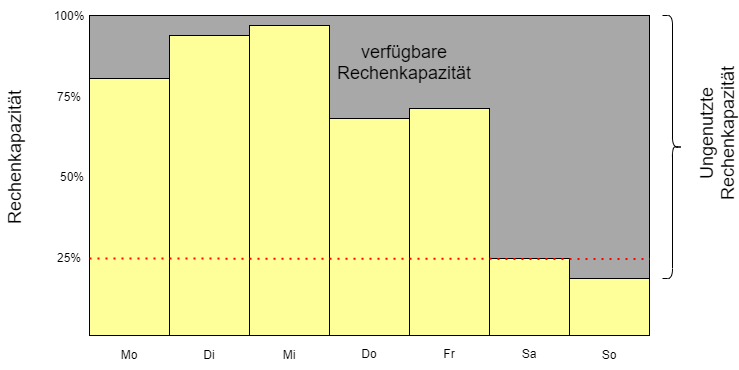
\includegraphics[scale=0.7]{sources/AutoCap Unused Capacity}\label{fig:AutoSca_Unused_Capacity}\\
    \textbf{Abbildung \autoref{fig:AutoSca_Unused_Capacity}:} Ungenutzte Ressourcen
    \footnote{Vgl. u.a.\cite{AMZ01}}
\end{center}

\subsubsection{Automatisiere das Hoch- und Herunterfahren von Dev/Test Umgebungen}
Grund: weil i.d.R., kein Entwickler 24/7 arbeitet.
Wie?: mit Tagging, Lambda oder mit Auto Scaling Groups.
%Wann ist es sinnvoll Systeme runterzufahren 

\subsubsection{(auto) Tiering }
Grund: nicht alle Dateien brauchen eine hohe Verfügbarkeit.
%Tiering, aber automatisch

\subsubsection{Automatisierung mit Lambda Funktionen}
Grund: einmal programmiert, funktioniert es für immer.
\\(To-Do:) Möglichkeiten untersuchen, bewerten und die passende Auswählen.
\subsubsection{Benachrigungen, wenn x\% Kapazität unterschreiten wurde}
Grund: um relevante Ereignisse nicht zu verpassen und rechtzeitig Maßnahmen zu ergreifen
%Limitierung 
%Quotas setzen? erweitern oder reduzieren / benachrichtigen aber auch eine Aktion durchführen 

%Turning stuffs OFF
%Lambda
\begin{comment}
AWS Lambda is a compute service. You can use it to run code without provisioning or managing servers. Lambda runs your code on a high-availability compute infrastructure. It operates and maintains all of the compute resources, including server and operating system maintenance, capacity provisioning and automatic scaling, code monitoring, and logging. With Lambda, you can run code for almost any type of application or backend service. 

Some benefits of using Lambda include the following:

You can run code without provisioning or maintaining servers.
It initiates functions for you in response to events.
It scales automatically.
It provides built-in code monitoring and logging via Amazon CloudWatch.
\end{comment}

%Data Pipeline
%CloudWatch

%Economic Performance?
%QUEUES

%NEVER forget your availability requirements, trying to optimize, first availability THEN cost...
%Do not use your DB for saving BLOB
warum ist das empfehlungswert?

\subsubsection{VERKAUFE DEINE Ungenutzte Kapazität in RI Marketplace}



  

 